\chapter{Code}
\label{chap: Code}

\section{相机内参标定实现}
利用MATLAB的“TOOLBOX\_calib”工具包在输入了标定图片之后会自动标定。标定得到的相机参数如图所示:

\begin{center}
    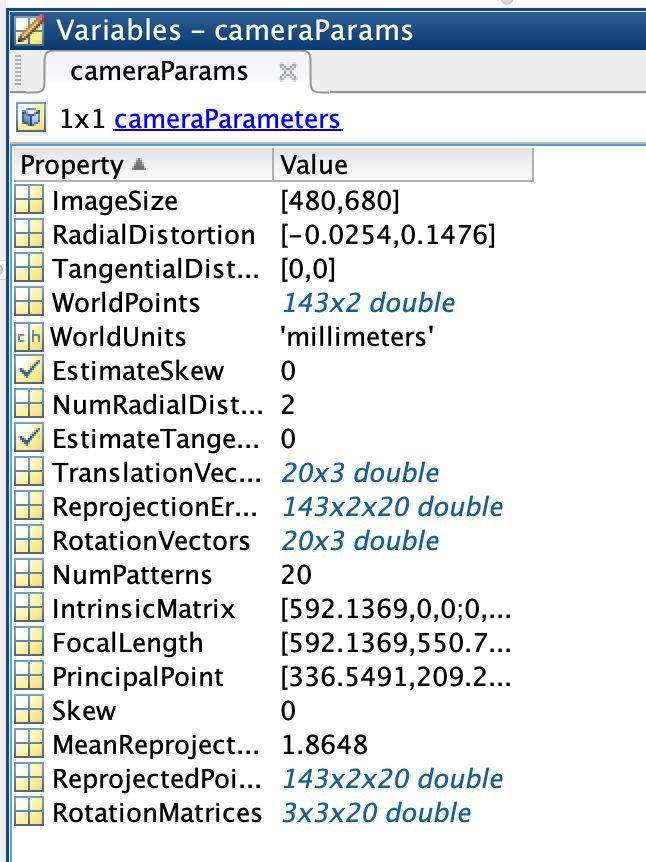
\includegraphics[width=0.4\textwidth]{figures/camera.png}
\end{center}

\section{去畸变}
MATLAB自带去除畸变的函数unditorImage,输入相机内参以及由该相机拍摄的图片即可获得去畸变处理后的图像

\begin{lstlisting}
I1 = undistortImage(I1,mycamera);
I2 = undistortImage(I2,mycamera);
I3 = undistortImage(I3,mycamera);
\end{lstlisting}


\section{特征点匹配}
在实际检测特征点的时候使用了SURF算子,对两张图片首先分别利用detectSURFFeatures函数检测图像的SURF特征点,该函数输入为需要提取特征的图像,返回提取得到的SURF特征点。然后利用extractFeatures函数对上一步提取得到的特征点计算描述向量用于之后的匹配。

extractFeatures函数的输入为图片以及对应的特征点,返回值为SURF描述子(特征描述向量)以及对应该描述子的点的位置。

\begin{lstlisting}
SURF_Pt_1 = detectSURFFeatures(rgb2gray(I1));
SURF_Pt_2 = detectSURFFeatures(rgb2gray(I2));
[features_1,validPoints_1] = extractFeatures(rgb2gray(I1),SURF_Pt_1);
[features_2,validPoints_2] = extractFeatures(rgb2gray(I2),SURF_Pt_2);
\end{lstlisting}

利用描述子做匹配的过程主要运用了matchFeatures函数,该函数输入为两个图像的特征描述子,返回的是匹配之后的匹配点的索引,index,其中index为n*2的矩阵,第一列对应第一张图像的匹配点的索引,第二列对应第二张图像的匹配点的索引。有了该索引,结合extractFeatures函数输出的描述向量对应点的位置,即可得到两张图片的匹配点。在匹配的过程中,为了降低outlier的比例,利用最佳匹配和第二好匹配的特征描述子距离比值进行筛选,对应于matchFeatures函数的’Maxratio’参数,在这里按照老师的建议设置为0.7。在得到了匹配点的位置之后就可以进行显示,显示函数为showMatchedFeatures